\chapter{Fundamentos teóricos}

El modelado y renderizado en 3D es posible gracias a una serie de técnicas
matemáticas y computacionales que permiten representar, manipular y visualizar
geometría en entornos virtuales. Copper se apoya principalmente en el modelado
mediante funciones de distancia con signo (SDF), el renderizado por \textit{ray
    marching} y el uso del estándar gráfico WebGPU. Este capítulo describe en
profundidad cada uno de estos fundamentos.

\section{Modelado tridimensional: Paradigmas y fundamentos}

El modelado tridimensional tradicional se basa en mallas poligonales, en las
que los objetos se representan mediante listas de vértices, aristas y caras
conectadas para formar la superficie. Herramientas como \textit{Blender},
\textit{Maya}, y \textit{3ds Max} utilizan este enfoque, que ofrece gran
flexibilidad para la edición y animación, pero que implica la gestión explícita
de la topología, el almacenamiento de grandes cantidades de datos y una
complejidad elevada para operaciones como la combinación de objetos o la
generación procedural de
geometría.

Como alternativa, existen los métodos de representación implícita,
especialmente los campos de distancia con signo (\textit{Signed Distance
    Fields, SDF}). Una SDF es una función $f(\vec{x})$ que, para cada punto
$\vec{x}$ del espacio, devuelve la distancia mínima a la superficie del objeto.
El signo indica si el punto está en el interior (negativo), sobre la superficie
(cero) o en el exterior (positivo). Este enfoque permite describir objetos
mediante expresiones matemáticas, simplificando la combinación y manipulación
de geometría compleja.

\section{Funciones de distancia con signo (SDF)}

Las SDF asignan a cada punto del espacio la distancia mínima a una superficie
implícita. Formalmente, para una función $f(\vec{x})$, la superficie se define
como el conjunto de puntos donde $f(\vec{x}) = 0$. Las SDF permiten describir
primitivas básicas como:

\begin{itemize}
    \item \textbf{Esfera}: $f_{esfera}(\vec{x}) = ||\vec{x} - \vec{c}|| - r$, donde $\vec{c}$ es el centro y $r$ el radio.
    \item \textbf{Caja}: $f_{caja}(\vec{x}) = ||\max(|\vec{x} - \vec{c}| - \vec{s}, 0)|| + \min(\max(d_x, \max(d_y, d_z)), 0)$, donde $\vec{s}$ es el tamaño.
    \item \textbf{Cilindro, cono, plano...}: Cada primitiva se expresa como una función matemática que determina la distancia a su superficie.
\end{itemize}

Las SDF pueden combinarse empleando operadores booleanos y suaves:

\begin{itemize}
    \item \textbf{Unión}: $f_{union}(a, b) = \min(a, b)$
    \item \textbf{Intersección}: $f_{inter}(a, b) = \max(a, b)$
    \item \textbf{Resta}: $f_{resta}(a, b) = \max(a, -b)$
    \item \textbf{Unión suave}: Interpolación entre distancias y colores para crear transiciones continuas.
\end{itemize}

Las SDF son especialmente potentes en contextos de modelado procedural y
generación fractal, permitiendo la composición jerárquica de formas y la
aplicación de transformaciones a nivel funcional. El cálculo de normales se
realiza mediante el gradiente de la función de distancia, habitualmente
aproximado numéricamente:

\begin{equation}
    \vec{n}(\vec{x}) \approx \nabla f(\vec{x}) = \left(
    f(\vec{x} + \epsilon \vec{i}) - f(\vec{x} - \epsilon \vec{i}),
    f(\vec{x} + \epsilon \vec{j}) - f(\vec{x} - \epsilon \vec{j}),
    f(\vec{x} + \epsilon \vec{k}) - f(\vec{x} - \epsilon \vec{k})
    \right)
\end{equation}

donde $\epsilon$ es un valor pequeño usado para la derivación numérica.

Las aplicaciones de las SDF abarcan desde el renderizado en tiempo real y la
simulación física (detección de colisiones) hasta la generación de terrenos y
la síntesis de geometría orgánica.

\subsection{Ventajas de las SDF frente al modelado poligonal}

\begin{itemize}
    \item \textbf{Compacidad}: Las SDF se definen por fórmulas matemáticas en lugar de listas de vértices, lo que reduce el espacio necesario para describir objetos complejos.
    \item \textbf{Facilidad de combinación}: La geometría puede combinarse empleando operadores matemáticos (unión, intersección, resta) de forma eficiente y expresiva.
    \item \textbf{Transformaciones geométricas}: Las transformaciones como traslación, rotación y escalado se aplican directamente sobre la función, facilitando la manipulación.
    \item \textbf{Cálculo de normales}: La normal en la superficie se obtiene como el gradiente de la función de distancia, lo que simplifica el cálculo de iluminación.
    \item \textbf{Flexibilidad}: Permiten crear transiciones suaves entre objetos mediante operadores suavizados, lo que es difícil de lograr con mallas.
\end{itemize}

\subsection{Limitaciones y retos actuales}

Más allá de las ventajas mencionadas, las SDF presentan retos abiertos en la
investigación y la ingeniería gráfica:

\begin{itemize}
    \item \textbf{Representación de formas arbitrarias}: Si bien las primitivas básicas se definen fácilmente, la conversión de mallas arbitrarias a SDF es un problema activo de investigación.
    \item \textbf{Eficiencia de evaluación}: El coste de evaluar funciones SDF complejas puede limitar su uso en escenas grandes o interactivas.
    \item \textbf{Animación y deformación}: La edición y animación de SDF requiere métodos específicos, como la interpolación funcional o la composición de transformaciones.
\end{itemize}

\section{Ray Marching}

El \textit{ray marching} es una técnica de renderizado que, utilizando la SDF,
avanza iterativamente un rayo en el espacio hasta aproximar la intersección con
una superficie implícita. El procedimiento puede describirse en los siguientes
pasos:

\begin{enumerate}
    \item Lanzar un rayo desde la cámara en una dirección determinada.
    \item Evaluar la SDF en la posición actual para obtener la distancia mínima a la
          superficie más cercana.
    \item Avanzar el punto a lo largo del rayo una distancia igual al valor obtenido.
    \item Repetir hasta que la distancia sea menor que un umbral (colisión con la
          superficie) o se alcance un límite de pasos o distancia máxima.
\end{enumerate}

Este método permite renderizar geometría definida implícitamente, como
fractales, superficies orgánicas, y escenas generadas proceduralmente.

\subsection{Ray Marching vs Ray Tracing}

\textbf{Ray tracing} tradicional calcula la intersección exacta entre el rayo y primitivas geométricas (esferas, triángulos, planos) resolviendo ecuaciones analíticas. Es eficiente para mallas y escenas donde la geometría está definida explícitamente.

En contraste, \textbf{ray marching} utiliza la SDF para aproximar la distancia
mínima a cualquier superficie, avanzando el rayo en pasos variables. Esto
permite renderizar geometría mucho más compleja y flexible, pero a costa de
necesitar muchas evaluaciones de la función y de aproximar, en vez de calcular
de forma exacta, la intersección.

\begin{itemize}
    \item \textbf{Ray tracing}: Preciso y eficiente para mallas, permite efectos avanzados (reflexión, refracción).
    \item \textbf{Ray marching}: Aproxima la superficie implícita, ideal para SDFs y fractales, más fácil de combinar con efectos procedurales y operaciones booleanas.
\end{itemize}

\subsection{Sphere Tracing}

La técnica de \textbf{sphere tracing}, introducida por Hart, es una variante
eficiente de ray marching. Utiliza la propia SDF para calcular el avance óptimo
en cada paso del rayo. En cada iteración, la distancia devuelta por la SDF se
interpreta como el radio de una esfera libre de obstáculos centrada en el punto
actual. Así, el rayo puede avanzar exactamente esa distancia sin riesgo de
atravesar ninguna superficie.

Sphere tracing es especialmente útil en escenas donde las funciones de
distancia son suaves y bien definidas, permitiendo renderizar geometría
compleja con costes computacionales bajos. Sin embargo, en superficies muy
delgadas o SDFs poco continuas, el algoritmo puede avanzar muy poco en cada
paso, reduciendo la eficiencia y generando artefactos
visuales.

\begin{figure}[H]
    \centering
    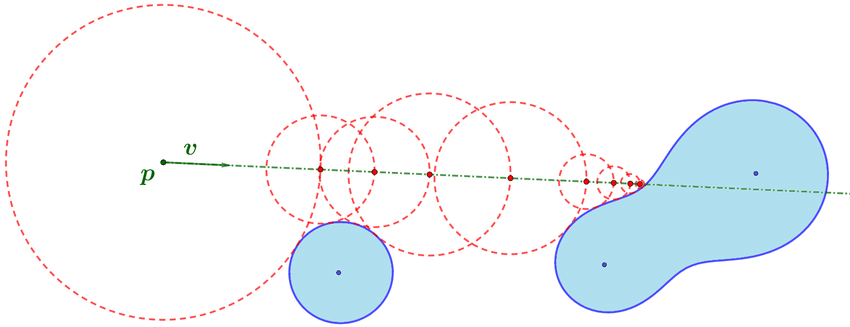
\includegraphics[width=0.6\textwidth]{sphere_tracing.png}
    \caption{Representación visual del algoritmo de sphere tracing, en el que cada círculo representa el rango libre de obstáculos determinado por la SDF.}
    \label{fig:sphere-tracing}
\end{figure}

\subsection{Limitaciones y consideraciones}

El ray marching y sphere tracing presentan los siguientes retos:

\begin{itemize}
    \item \textbf{Precision y aliasing}: El umbral de colisión y el número de pasos afectan la calidad de la imagen y pueden causar aliasing o superficies rugosas.
    \item \textbf{Superficies delgadas}: Si la SDF varía abruptamente o la superficie es muy fina, el avance óptimo se reduce y el número de pasos aumenta significativamente.
    \item \textbf{Efectos avanzados}: Efectos como la refracción y la reflexión requieren múltiples rayos y aumentan el coste computacional.
    \item \textbf{Desempeño}: El rendimiento depende de la complejidad de las funciones SDF y del número de objetos en escena.
\end{itemize}

\section{WebGPU: Acceso moderno a la GPU}

WebGPU es un estándar gráfico de nueva generación que proporciona acceso
eficiente y multiplataforma a la GPU, tanto en navegadores como en aplicaciones
nativas. WebGPU surge como respuesta a las limitaciones de APIs tradicionales
como OpenGL y DirectX, ofreciendo mayor control sobre el hardware, mejor
rendimiento y portabilidad.

\subsection{Motivación y principios de diseño}

WebGPU fue diseñado para proporcionar:

\begin{itemize}
    \item \textbf{Multiplataforma}: Disponible en Windows, Linux, macOS y en navegadores modernos (Chrome, Firefox, Safari).
    \item \textbf{Eficiencia}: Permite describir el flujo de datos entre la CPU y la GPU mediante buffers y pipelines, minimizando el coste de las llamadas de función y la sobrecarga del sistema.
    \item \textbf{Seguridad y portabilidad}: WebGPU abstrae detalles específicos del hardware, garantizando que el mismo código funcione en diferentes dispositivos y plataformas.
    \item \textbf{Modelo explícito}: El usuario configura directamente los recursos (buffers, texturas, pipelines) y controla el ciclo de vida de los datos, permitiendo optimizaciones avanzadas.
\end{itemize}

En contraste con OpenGL/WebGL, WebGPU obliga a definir explícitamente los
recursos y su uso, lo que mejora la seguridad y el rendimiento pero requiere
una mayor comprensión del modelo de GPU.

\subsection{Conceptos clave de WebGPU}

De acuerdo con la guía, los fundamentos de WebGPU incluyen:

\begin{itemize}
    \item \textbf{Buffers}: Áreas de memoria para almacenar datos como vértices, índices y uniformes.
    \item \textbf{Textures}: Imágenes y mapas de datos que pueden ser leídos y escritos por la GPU.
    \item \textbf{Bind Groups}: Conjuntos de recursos que se vinculan a los shaders, permitiendo el acceso eficiente a datos en la GPU.
    \item \textbf{Pipelines}: Describen la secuencia de operaciones gráficas, incluyendo shaders, estados de rasterización y configuración de recursos.
    \item \textbf{Shaders}: Programas ejecutados en la GPU que transforman datos y calculan colores de píxeles.
    \item \textbf{Command Buffers}: Secuencias de instrucciones que la GPU ejecuta para renderizar o procesar datos.
\end{itemize}

WebGPU utiliza el lenguaje WGSL (\textit{WebGPU Shading Language}) para la
programación de shaders, ofreciendo una sintaxis moderna y expresiva adaptada a
las necesidades de la computación gráfica actual.

\section{Shaders y lenguaje WGSL}

Los \textbf{shaders} son programas que ejecutan operaciones matemáticas en la
GPU para transformar vértices, calcular colores y simular efectos visuales. En
WebGPU, los shaders se escriben en WGSL (\textit{WebGPU Shading Language}), un
lenguaje moderno diseñado para expresar funciones de distancia, operadores
booleanos, cálculos de iluminación y efectos visuales de forma eficiente.

\begin{itemize}
    \item \textbf{Vertex shaders}: Transforman posiciones y atributos de vértices.
    \item \textbf{Fragment shaders}: Calculan el color final de cada píxel, aplicando modelos de iluminación como Blinn-Phong, efectos de sombras y combinaciones de SDF.
\end{itemize}

WGSL permite aprovechar la arquitectura de la GPU para realizar renderizado en
tiempo real, combinando eficiencia y expresividad.

\section{Herramientas auxiliares}

El desarrollo de aplicaciones gráficas requiere gestionar ventanas, entrada de
usuario y la interfaz gráfica. Copper utiliza las siguientes herramientas:

\begin{itemize}
    \item \textbf{GLFW}: Biblioteca multiplataforma para la gestión de ventanas y eventos~\cite{glfw-docs}.
    \item \textbf{ImGui}: Sistema de interfaz gráfica inmediata para la manipulación interactiva de primitivas y parámetros de escena~\cite{imgui-docs}.
    \item \textbf{GLM}: Biblioteca matemática para operaciones con vectores y matrices~\cite{glm-docs}.
    \item \textbf{CMake}: Herramienta de compilación y gestión de dependencias~\cite{cmake-docs}.
\end{itemize}

Estas herramientas proporcionan la infraestructura básica para la interacción y
visualización dentro del entorno de Copper.